\documentclass[12pt]{article}
\usepackage{hyperref, graphicx, titling}
\usepackage[a4paper, total={6in, 9in}]{geometry}
\title{Lab 6 Submission}

\author{Ethan Vosburg\\
    Cal Poly SLO \\
    Fall 2023\\
    CPE 133\\
    Instructor: Gary Perks
}

\begin{document}

\maketitle

\newpage

\section{Introduction}

The goal of this lab was to design and program a logic circuit that detects a programmed sequence. This lab was a success and I was able to complete all of the tasks.

\section{Video of Working Project}

Linked here is a video of the working project: \href{https://youtu.be/sftY2CiYkgA}{Project Video}

\section{Simulation}

\begin{figure}[h]
    \centering
    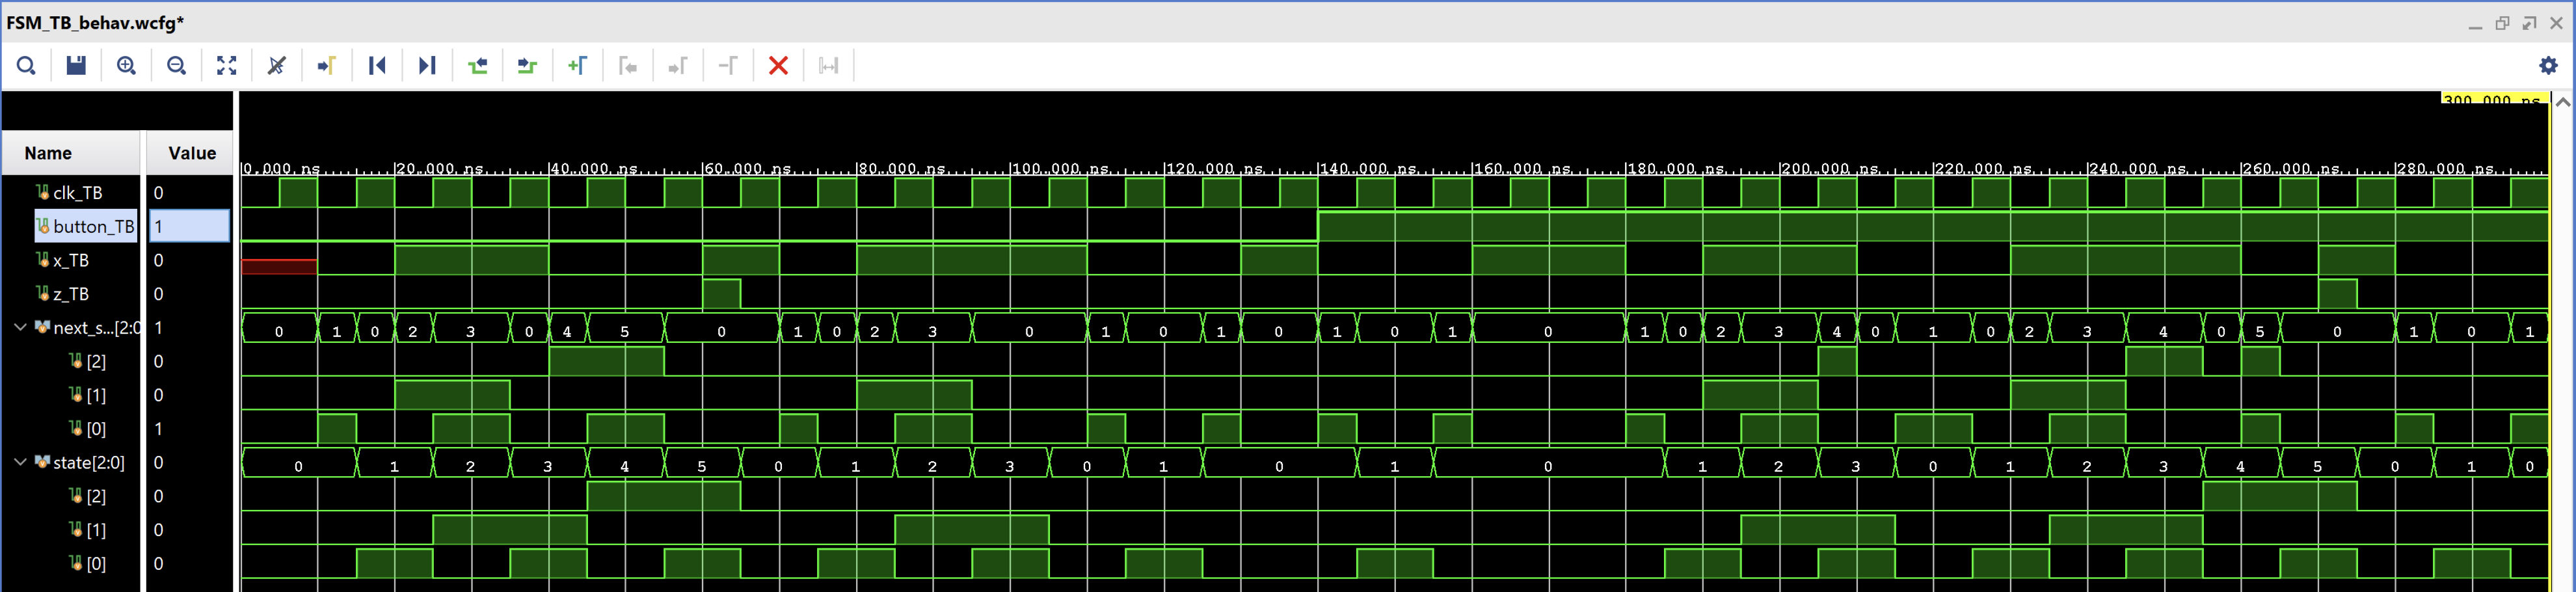
\includegraphics[width=.8\textwidth]{Figures/CPE 133 Lab 6 Simulation.png}
    \caption{Vivado Simulation}
    \label{fig:simulation}
\end{figure}

\section{Elaborated Design}

Presented below is the elaborated design of the project generated by Vivado.

\begin{figure}[h]
    \centering
    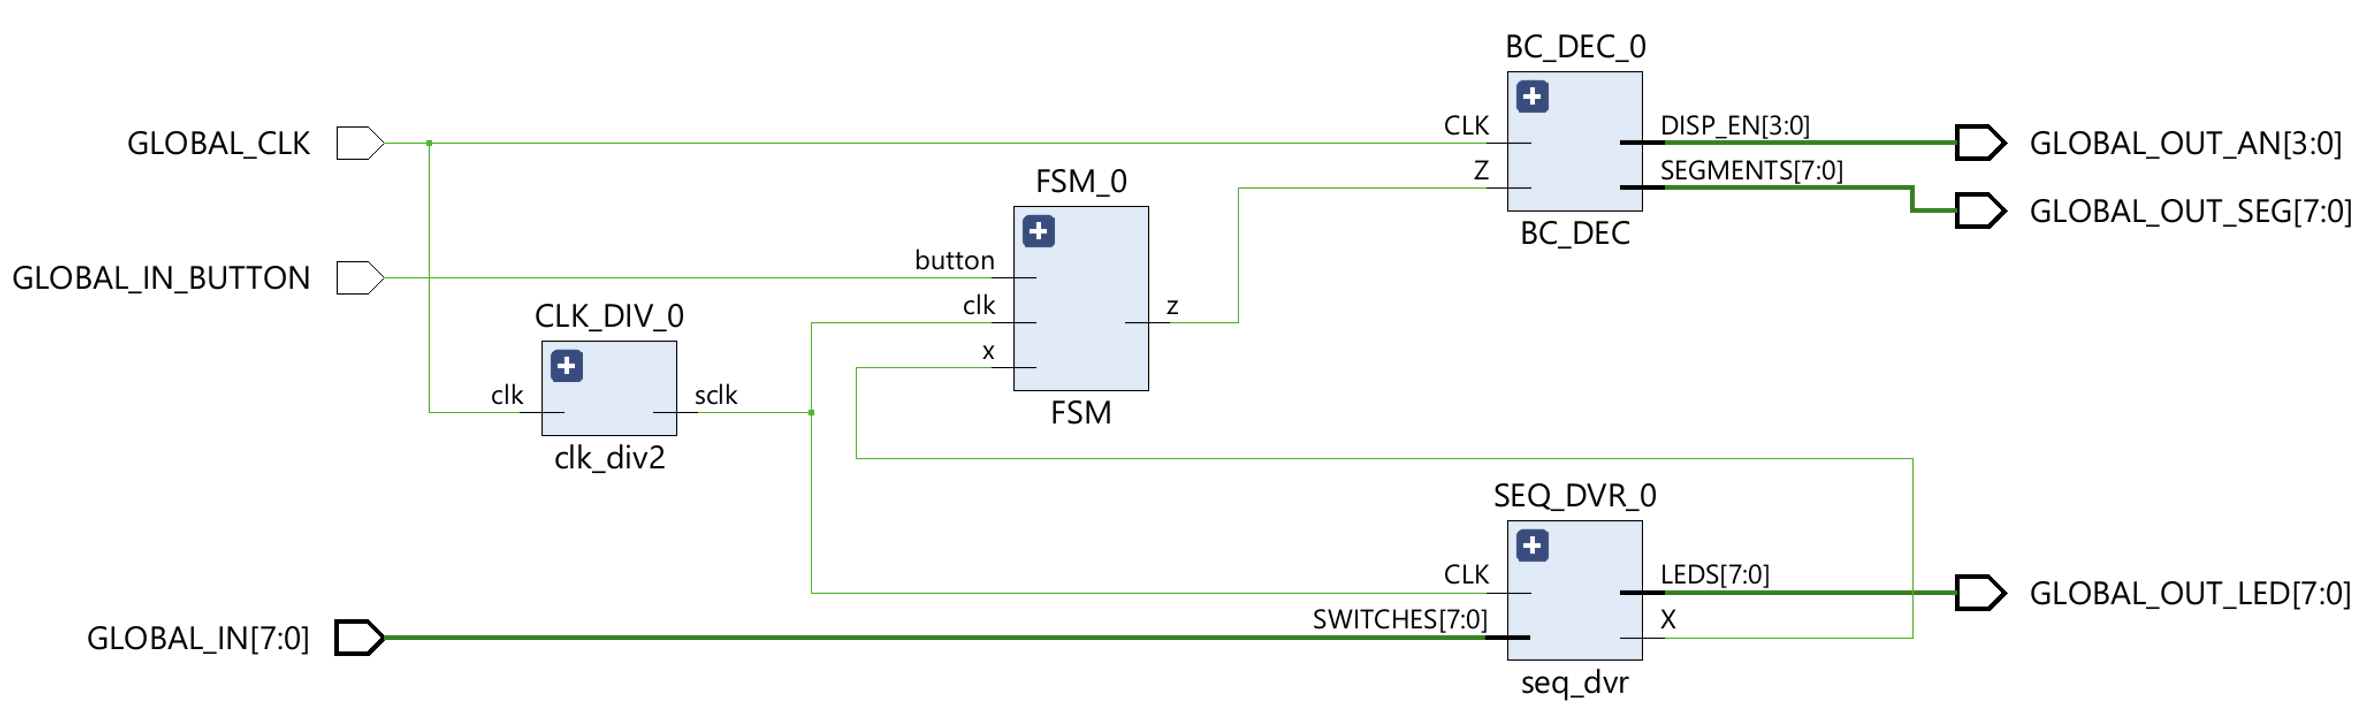
\includegraphics[width=.95\textwidth]{Figures/CPE 133 Lab 6 Elaborated Design.png}
    \caption{Elaborated Design}
    \label{fig:elaborateddesign}
\end{figure}

\newpage

\section{Error Log}

There were no errors or significant warnings in the Vivado log as shown below.

\begin{figure}[h]
    \centering
    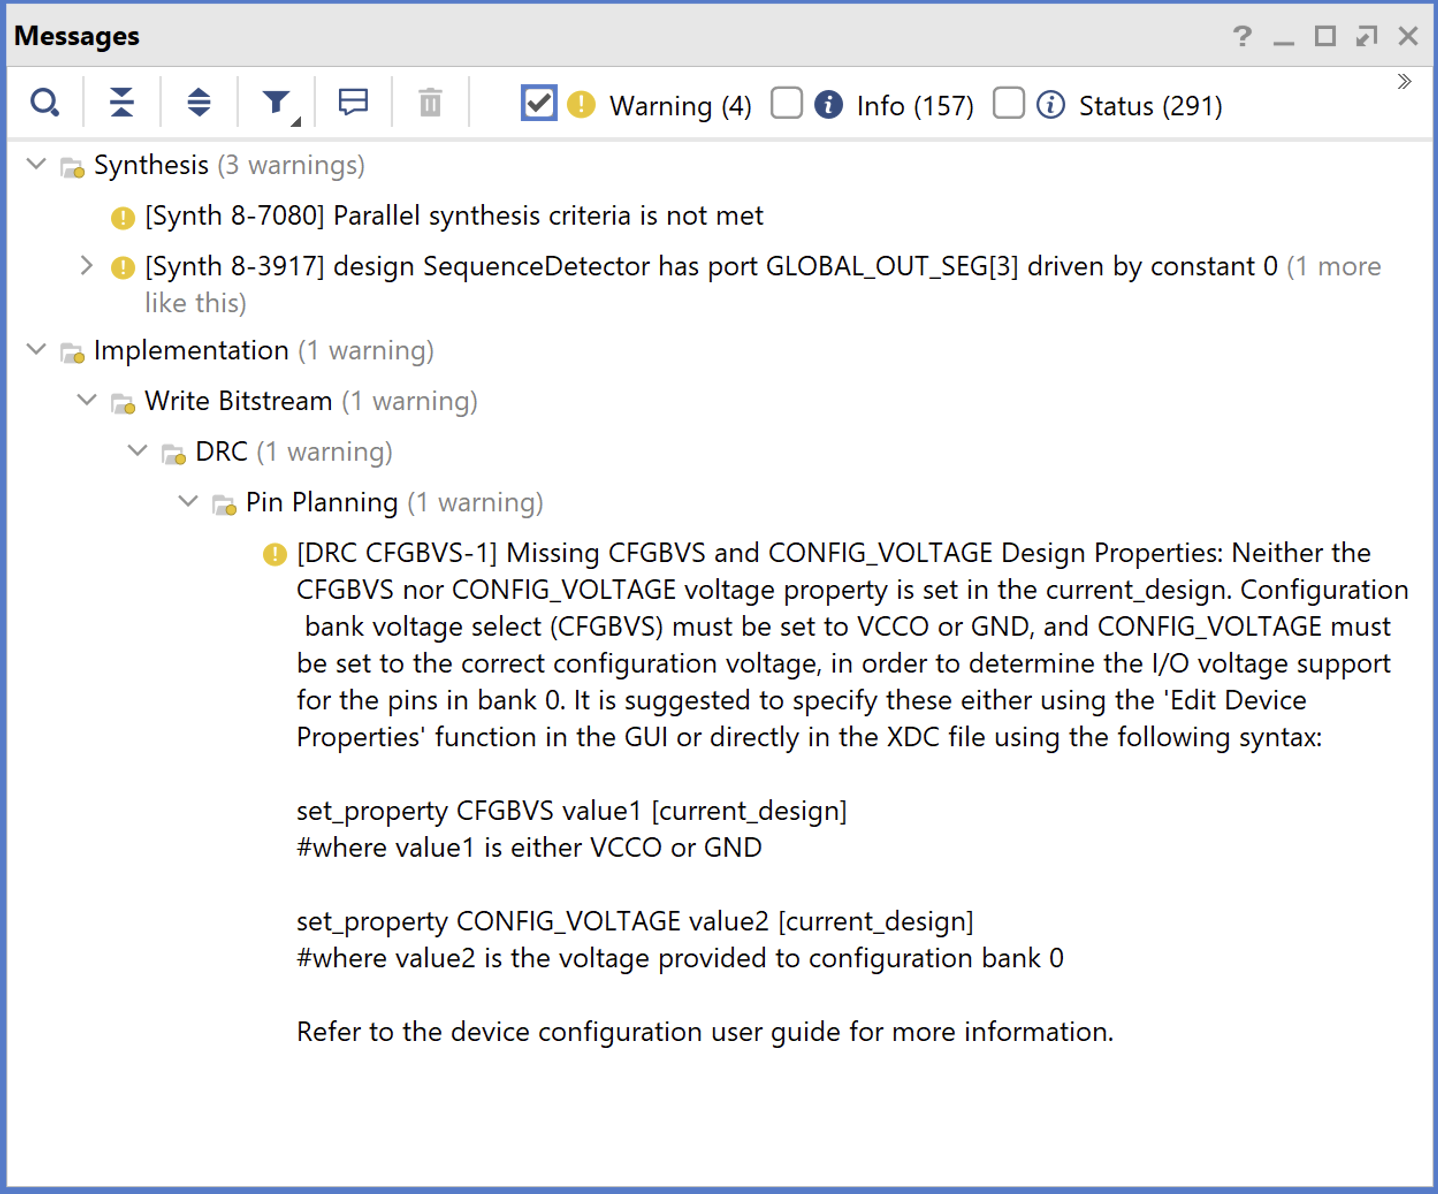
\includegraphics[width=.8\textwidth]{Figures/CPE 133 Lab 6 Error Log.png}
    \caption{Error and Warning Log}
    \label{fig:warninglog}
\end{figure}



\end{document}